\newpage
\section{Fault-Tolerance Design}
\label{sec:ftDesign}
This section describes the design of the archive service in case of different kinds of failures. The system being part of a large distributed system,
faces different difficult situation which must be handled for a stable application. Table \ref{table:probServices} lists the possible errors which 
may occur with a brief description, i.e., network issues, failure of a 
dependent service, sudden termination of the archive service. 
\begin{longtable}{|p{4cm}|p{10cm}|}
    \hline
        \textbf{Errors}  & \textbf{Description}\\
    \hline
        Network glitches & The communication between the services
        happen via a network (e.g., HTTP, RPC) in the MARS system. It is a possibility that the connection is not available for a small period due to network problems.
        This phenomenon would lead the archive service to fail even though all the services are functioning.\\
    \hline
        Failure of a dependent service & There is a possibility that a service which the archive service is dependent upon goes down temporarily due to an unexpected
        failure or is in maintenance. The failure of the dependent service to reply also generates an error in the Archive service.\\
    \hline
        Sudden failure of the Archive service & Like all the other services the Archive service is also prone to getting an unexpected restart. 
        This restart causes the running job to stop and lose its current progress.\\    
    \hline
    \caption{Possible errors which could occur in the Archive service}
    \label{table:probServices} 
\end{longtable}

Figure \ref{fig:activityFailure} illustrates the activity diagram which describes the Archive service's design that recovers from errors mentioned in
Table \ref{table:probServices}. The main strategy for the failure mitigation is to re-run the process again from the beginning once an error occurs. 
A programmer can configure the number of restarts and cumulative wait time for the restart. It is designed in such a way so that the service avoids a deadlock situation with infinite restarts.


\begin{figure}[H]
    \centering 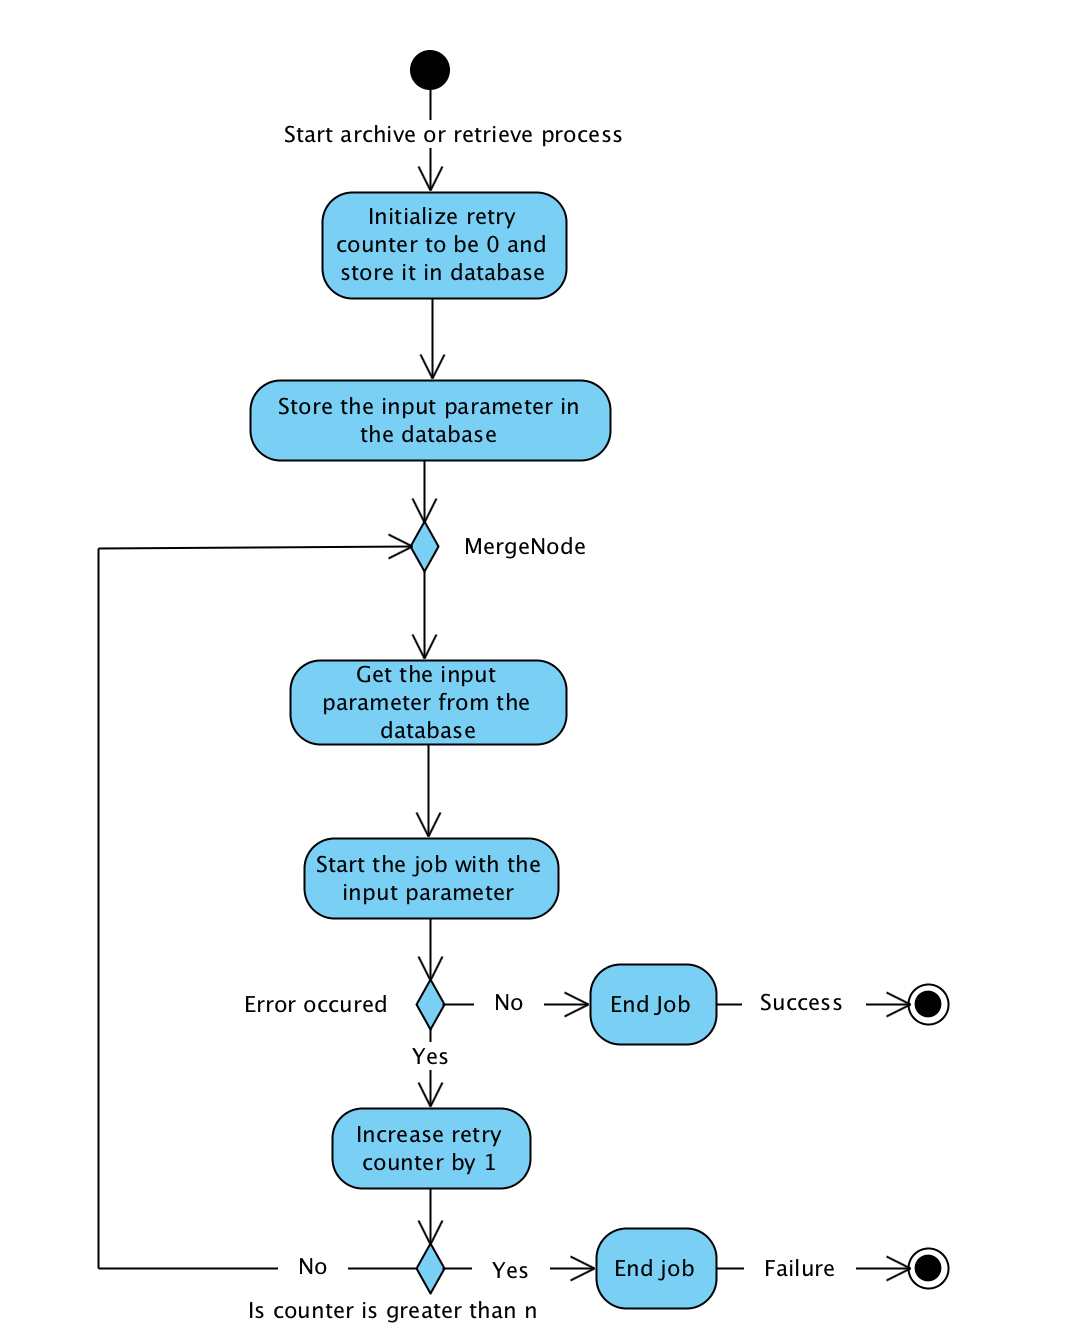
\includegraphics[scale=0.6]{grafiken/activityFailure.png}
    \caption{Activity Diagram for failure mitigation for the Archive service}
    \label{fig:activityFailure}
\end{figure}
